\documentclass[10pt]{article}

\usepackage{polski}
\usepackage{graphicx}
\usepackage{hyperref}
\graphicspath{{images/}}

\usepackage{geometry}
\newgeometry{tmargin=4cm, bmargin=4cm, lmargin=3.2cm, rmargin=3.2cm}

\usepackage{fancyhdr}
\pagestyle{fancy}



\begin{document}

\begin{titlepage}


\begin{center}

  \LARGE \textsc{Politechnika Wrocławska}\\
  \vspace*{0.2cm}
  \Large \textsc{Wydział Informatyki i Telekomunikacji}\\
  \vspace*{0.4cm}
  \centering
\includegraphics[width=0.2\textwidth]{WITlogo.png}\\
  \vspace*{0.2cm}
  \vspace*{2cm}

  \centerline{\rule{\textwidth}{1.2pt}}
  \vspace{0.4cm}
  \Huge\textbf{Metody i Systemy Decyzyjne}
  \centerline{\rule{\textwidth}{1.2pt}}
  \vspace{1cm}
  \LARGE Sprawozdanie z laboratorium\\
  \vspace{3.5cm}
  \textsc{Autor}\\
  \vspace{0.2cm}
  \textbf{Bartosz Kalisz}\\
  \vspace{0.1cm}
  \Large nr albumu: \textbf{259206}\\
  \vspace{0.1cm}
  kierunek: \textbf{Informatyka Stosowana}

  \vspace*{\fill}
  \Large \textit{\today}

 \end{center}


\end{titlepage}


\begin{abstract}
Celem projektu jest przeanalizowanie darmowych dostępnych punktów wi-fi w mieście Gdańsk oraz znalezienie optymalnego miejsca do utworzenia kolejnej takiej placówki.  
\end{abstract}

\section{Wstęp -- sformułowanie problemu}
\label{sec:wstep}

Władze miasta potrzebują przewidzieć gdzie postawić następną sieć darmowego wi-fi, aby jak najwięcej ludzi mogło z niej skorzystać, uwzględniając już istniejące punkty. Pozwoli to na większe zadowolenie wśród mieszkańców miasta. Badania będą przeprowadzone w oparciu o dwie zmienne: współrzędne geograficzne oraz wielkość przepływu danych w już istniejących placówkach.  

\begin{itemize}
    \item \textbf{współrzędne geograficzne} - para liczb jednoznacznie określająca położenie danego miejsca na świecie
    \item \textbf{wielkość przepływu} - łączna ilość pobranych i przesłanych danych w danej sieci wi-fi.   
\end{itemize}

\section{Opis rozwiązania} 
 Dane pobrałem ze strony \url{https://www.gdansk.pl/otwarte-dane?show=data&id=wifi-gdansk-2020&s=byGroup&i=urzad-miejski}. Korzystając z biblioteki pandas utworzyłem ramkę danych. Każdy rekord zawierał informacje o pojedynczej sieci wi-fi w mieście Gdańsk: nazwa placówki, łączna ilość wysłanych danych, łączna ilość pobranych danych. Za pomocą biblioteki geocoder zamieniłem nazwy obiektów w Gdańsku na interesujące mnie dane - współrzędne. Wykresy dla sformułowanych problemów zrobiłem głównie  za pomocą matplotlib. Wielu obliczeń dokonywałem za pomocą biblioteki numpy, natomiast funkcję zoptymalizowałem dzięki scipy . 

\section{Rezultaty obliczeń}

\subsection{Plan badań}

Na początku ustaliłem funkcję celu w postaci : 


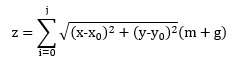
\includegraphics[width=0.4\linewidth]{rownanie.png}
\end{center}
gdzie x,y to współrzędne, j - liczba punktów wi-fi, w - transfer wychodący, natomiast p to transfer przychodzący. Taka funkcja, miała na celu znalezienie punktu, którego suma odległości od wszystkich punktów pomnożona przez ich przepływ danych jest największa. Takie miejsce jest najlepsze, ponieważ pokazuje nam największe zapotrzebowanie. Na końcu zdefiniowałem granice na podstawie współrzędnych Gdańska, aby żaden punkt nie wypadł poza obszar miasta.


\subsection{Wyniki obliczeń}
\subsubsection{Wykres zależności zapotrzebowania na sieć wi-fi od współrzędnych}
\begin{center}
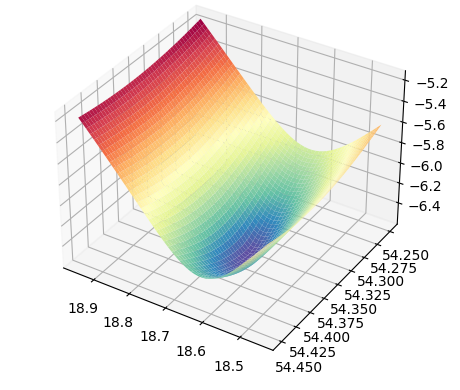
\includegraphics[width=0.65\linewidth]{wykres_1.png}
\end{center}
\begin{center}
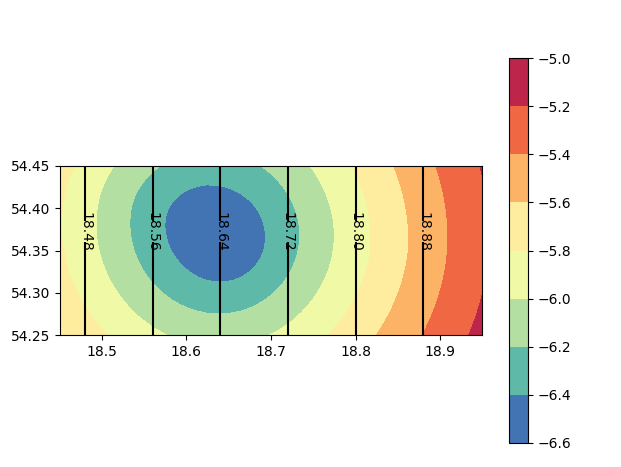
\includegraphics[width=0.65\linewidth]{wykres_2.png}
\end{center}
Na powyższym wykresie wyraźnie widać określoną zależność między współrzędnymi. Wokół największego skupiska placówek z darmowym wi -fi jest średnio największy przepływ danych, łączący się z średnim najmniejszym odstępem poszukiwanego miejsca od podanych punktów.

\section{Wnioski}
Na podstawie analizy powyższych zależności można wysnuć wnioski. 
\newline \textbf{Potrzeba na kolejną sieć darmowego wi -fi } jest największa w miejscach najbardziej odwiedzanych, paradoksalnie tam gdzie istnieje już najwięcej takich placówek. Zagłębiając się jednak w ten temat dochodzimy do wniosku że nic w tym dziwnego. Miejsca najbardziej odwiedzane generują największy przepływ danych i to właśnie tam potrzeba jest na kolejne takie miejsca, w celu odciążenia. Nie ma sensu stawiać sieci wi-fi gdzieś na granicach miasta, gdzie zaludnienie jest o wiele mniejsze i choć średnio odległość między pozostały placówkami jest duża to przepływ danych w takim miejscu byłby znikomy ze względu na małą liczbę korzystających użytkowników.


\end{document}
